\chapter[Reconstruction of cholangiocarcinoma microevolution through rapid research autopsy]{Reconstruction of cholangiocarcinoma microevolution through rapid research autopsy\footnote{This chapter previously published as: Krook MA\cofirst, Bonneville R\cofirst, \textit{et al}. Tumor heterogeneity and acquired drug resistance in FGFR2 fusion-positive cholangiocarcinoma through rapid research autopsy. \textit{CSH Molecular Case Studies} 2019, 5:a004002.}}
\label{ch:240}

\section{Introduction}
Cholangiocarcinoma is an aggressive and deadly rare cancer arising from bile duct epithelial cells with a five-year overall survival rate of less than 2\% for advanced stage disease \cite{pdqchol2002,razumilava2014}. Most patients with cholangiocarcinoma present with metastatic unresectable cancer, thus precluding curative therapy \cite{razumilava2014,valle2010}. Given its poor prognosis and limited treatment options beyond first-line chemotherapy, development and optimization of novel therapies for cholangiocarcinoma is urgently needed.

The fibroblast growth factor receptor (FGFR) signaling pathway is aberrantly activated in approximately 20\% of cases of intrahepatic cholangiocarcinoma through various genomic alterations including point mutations, copy number amplifications, and gene fusions \cite{roychowdhury2011_ngs,wu2013}. Extending beyond cholangiocarcinoma, alterations in the FGFR signaling pathway have been reported in non-small cell lung carcinoma, endometrial cancer, and urothelial cancer \cite{krook2020}. Currently, several tyrosine kinase inhibitors, covalent and non-covalent, non-selective and selective FGFR inhibitors are being assessed clinically in patients with metastatic cancer and have shown early responses in those patients with metastatic FGFR-mutant cancers \cite{andre2013,angevin2013,gozgit2012,javle2018,paik2017,tabernero2015}. While genomic alterations in \textit{FGFR} correlated with initial clinical responses to FGFR inhibitors, multiple secondary mutations in \textit{FGFR} and other cellular signaling pathways have been identified in patients after treatment with FGFR inhibitors. Thus, elucidating the various acquired mechanisms of drug resistance to FGFR inhibitors will be critical for the development of new therapies to overcome resistance and improve the outcome of patients with FGFR-mutant cancers.

Tumor heterogeneity has been shown to negatively impact therapeutic response and contribute to treatment resistance in cancer patients, and thus it remains a major impediment to cancer treatment \cite{bedard2013,burrell2014,dexter1986,fisher2013,heppner1989}. Both genetic and epigenetic mechanisms within the tumor itself as well as changes in the tumor microenvironment can drive the development of tumor heterogeneity \cite{heng2009,junttila2013,meacham2013}. Genomic characterization of primary and recurrent/metastatic tumors from the same patient has further demonstrated spatial and temporal intrapatient tumor heterogeneity (ITH) \cite{bedard2013}. Recent studies have evaluated ITH and clonal evolution through next-generation sequencing (NGS) methods, demonstrating the critical role of these processes in recurrence and development of therapeutic resistance in urothelial carcinoma, renal cell carcinoma, and acute myeloid leukemia \cite{ding2012,faltas2016,gerlinger2012,gerlinger2014}. Studies like these, however, are limited in cholangiocarcinoma.

To date, the genomic landscape of cholangiocarcinoma has been largely characterized through tumor biopsies and surgical specimens and, therefore, may not accurately reflect the complex and heterogeneous nature of metastatic and drug-resistant disease \cite{farshidfar2017,jusakul2017,ruzzenente2016,zou2014}. Recently, Goyal \textit{et al} \cite{goyal2017} evaluated three patients with FGFR-fusion positive cholangiocarcinoma who received the FGFR inhibitor BGJ398. Targeted gene panel sequencing using the commercial Guardant360\textsuperscript\textregistered{} assay revealed an \textit{FGFR2} V564F gatekeeper mutation in plasma circulating tumor DNA (ctDNA) of all three patients and several additional FGFR2 mutations in two of the patients. One patient consented to rapid research autopsy and this enabled the procurement of multiple metastatic tumors for genomic profiling with the FoundationOne\textsuperscript\textregistered{} assay (315 gene panel) to study acquired drug resistance to the drug BGJ398. This study successfully demonstrated the role of acquired mutations in resistance to BGJ398. It also demonstrated heterogeneity at time of autopsy since 8 of 12 tumor samples assessed lacked a secondary mutation in \textit{FGFR2}. However, there are more than ten FGFR inhibitors in active drug development in clinical trials, and mechanisms of resistance for each of these drugs remain a significant gap in knowledge. Prior research on acquired resistance mutations in \textit{KIT}, \textit{ABL1}, and \textit{ALK} oncogenes with their respective kinase inhibitors, demonstrates that cross-resistance and sensitivity for secondary mutations varies widely, and therefore understanding resistance profiles for other FGFR inhibitors will be essential. Further, evaluating additional patients receiving other FGFR inhibitors with an expanded scope of whole exome (\textgreater{}~20,000 genes) will be critical to characterizing clonal heterogeneity and evolution with FGFR inhibitors.

In the current work, we present a patient with metastatic cholangiocarcinoma harboring a novel \textit{FGFR2-CLIP1} gene fusion who demonstrated a partial response followed by disease progression while on treatment with the FGFR-selective kinase inhibitor, INCB054828\footnote{INCB054828 has since been assigned the USAN generic name pemigatinib.}. Through rapid research autopsy of this patient and whole exome sequencing (WES) of his metastatic cancer, we identified four unique tumor subclones and elucidated their evolution from the normal ancestral cell. Furthermore, we identified a post-treatment secondary kinase mutation in \textit{FGFR2} present in a single metastatic tumor sample, and characterized its impact on sensitivity to a variety of FGFR inhibitors \textit{in vitro}. The results of our \textit{in vitro} drug sensitivity studies suggest that this mutation conferred resistance to INCB054828 in this patient and thus may have potential as a clinically useful biomarker of resistance. Importantly, characterizing tumor heterogeneity and the ability to detect clonal evolution in patients will facilitate approaches to prevent or overcome treatment resistance and disease recurrence.

\section{Materials and Methods}
\label{sec:240:methods}
\subsection{Research autopsy and patient samples}
\begin{figure}[htp]
    \begin{center}
        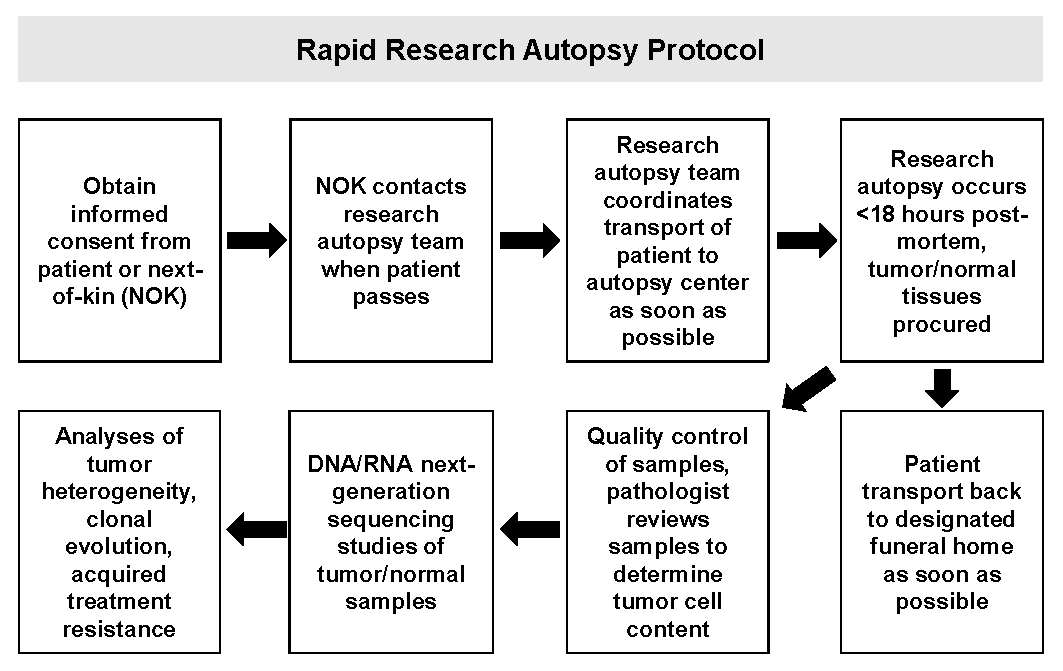
\includegraphics[width=0.85\textwidth,keepaspectratio]{images/240/autopsy_flowchart}
    \end{center}
    \caption{Overview of research autopsy protocol.}
    \label{fig:240:autopsy_flowchart}
\end{figure}
The patient consented to an IRB-approved study for high-throughput sequencing of tumor and normal specimens (OSU-13053, NCT02090530) at the James Cancer Hospital and The Ohio State University (Section~\ref{ssec:intro:heterogeneity_methods}). OSU-SpARKFuse, a targeted RNA based next generation sequencing assay to detect gene fusions, and a targeted DNA sequencing assay to detect single nucleotide variations were performed on tumor biopsy specimens as previously described \cite{samorodnitsky2015_ngs,reeser2017}. The patient also consented to a body donation study (Figure~\ref{fig:240:autopsy_flowchart}). Upon death of this patient, next of kin informed the research team, who arranged for transportation to the OSU Regional Autopsy Center and the autopsy was performed 8 hours post-mortem. Guided by radiographic scans, all visible malignant as well as adjacent normal tissues were collected and frozen in Optimal Cutting Temperature (OCT) compound. Following the autopsy, the patient was returned to the funeral home.

\subsection{Histology}
Freshly collected tumor biopsy and autopsy samples were immediately embedded and frozen in OCT compound (Thermo Fisher\textsuperscript\textregistered{}). Frozen sections were cut from tumor biopsy and autopsy samples at 5µm on a Leica\textsuperscript\texttrademark{} Cryostat CM1950 for H\&E staining. A board-certified pathologist reviewed representative slides for each tumor block for estimated tumor content.

\subsection{Whole exome sequencing}
Genomic DNA was extracted from frozen tumor biopsy samples and tumors collected during autopsy using the \mbox{QIAamp}\textsuperscript{\textregistered} DNA Mini Kit (Qiagen\textsuperscript{\textregistered}). The \mbox{QIAamp} DNA Mini Blood Kit (Qiagen) was used to extract genomic DNA from blood. Whole exome sequencing was performed as described below. Briefly, the KAPA HyperPrep\textsuperscript\texttrademark{} Kit (Roche\textsuperscript\texttrademark{}) was used for library preparation, and libraries were enriched using the xGen\textsuperscript\texttrademark{} Exome Research Panel v1.0 from Integrated DNA Technologies (IDT\textsuperscript\texttrademark{}). 2\texttimes{}150 bp paired-end sequencing was performed on an Illumina\textsuperscript\textregistered{} HiSeq\textsuperscript\textregistered{} 4000 at The Genomics Services Laboratory at Nationwide Children's Hospital (Columbus, Ohio).

\subsection{Sequence alignment and variant calling}
\label{ssec:240:alignment_variant_calling}
All bioinformatics analyses were performed using the Oakley supercomputer at the Ohio Supercomputer Center \cite{Oakley2012}. Alignment of whole exome sequencing data to the human genome version hg19 \cite{lander2001} was performed BWA \cite{bwa} version 0.7.14. Duplicate reads were removed with Picard \cite{Picard2019toolkit} version 2.3.0. Picard and GATK \cite{mckenna10} version 3.5 were used to perform quality recalibration and local realignment around indels. Single nucleotide variation (SNV) and indel calling were performed with VarScan2 \cite{varscan2} version 2.3.9. Raw somatic variant calls were filtered using bam-readcount \cite{bamreadcount} as follows:
\begin{table}[H]
	\centering
	\begin{tabular}{l|l}
		Filter                                   & Threshold  \\
		\hline
		$P$ (Fisher's exact test)                & $\le 0.05$ \\
		Average quality of alt-supporting reads  & $\ge 22$   \\
		Variant allele fraction                  & $\ge 6\%$  \\
		Average mutation distance to 3' read end & $\ge 0.24$ \\
		Mismatch rate in alt-supporting reads    & $\le 0.04$ \\
		Average sum of base quality mismatches   & $\le 100$
	\end{tabular}
	\label{table:240:somaticSNVfilter}
\end{table}
\noindent Germline SNVs (used for CNV calling) were filtered as follows:
\begin{table}[H]
	\centering
	\begin{tabular}{l|l}
		Filter                                   & Threshold  \\
		\hline
		$P$ (Fisher's exact test)                & $\le 0.1$  \\
		Average quality of alt-supporting reads  & $\ge 22$   \\
		Variant allele fraction                  & $\ge 6\%$  \\
		Average mutation distance to 3' read end & $\ge 0.24$ \\
		Mismatch rate in alt-supporting reads    & $\le 0.04$ \\
		Average sum of base quality mismatches   & $\le 100$
	\end{tabular}
\end{table}
\noindent To filter indels in difficult-to-call repetitive regions, RepeatFinder (packaged with MANTIS \cite{kautto17}) was used to generate a list of all regions in hg19 at least 4 bp in length that contained a 1 to 5-mer repeating sequence (Section~\ref{ssec:msilandscape:mantis}). Somatic indels were then filtered as follows:
\begin{table}[H]
	\centering
	\begin{tabular}{l|l}
		Filter                                   & Threshold  \\
		\hline
		$P$ (Fisher's exact test)                & $\le 0.05$ \\
		Variant allele fraction                  & $\ge 6\%$  \\
		Not in repetitive region & \\
	\end{tabular}
\end{table}

SNVs and indels were annotated using ANNOVAR \cite{annovar} (revision \#11f4bb, 2016-02-01) (Supplemental File~S\thechapter{}.1). Putative driver mutation analysis was performed with CRAVAT \cite{douville2013} version 5.2.4, using the CHASM \cite{carter2009}, algorithm version 3.1. Tumor mutational burden (TMB) was computed as the sum of all called somatic SNVs and indels within the capture region in each sample, divided by the size of the capture region (\textapprox{}38.9~Mb). Microsatellite instability (MSI) testing was performed with MANTIS \cite{kautto17} (Chapter~\ref{ch:msilandscape}) using the recommended threshold of 0.4 to call MSI and a set of 2,539 whole exome microsatellite loci (Section~\ref{ssec:msilandscape:loci_selection}). Mutational signatures were called with deconstructSigs \cite{rosenthal16} version 1.8.0 using the COSMIC Mutational Signatures set \cite{cosmic_ms}, exome2genome trinucleotide frequency correction, and otherwise default settings (Supplemental File~S\thechapter{}.2).

\subsection{Copy number variation analysis}
\label{ssec:240:cnv_methods}
Copy number variation (CNV) calling was performed using FALCON \cite{falcon} version 0.2, utilizing germline tumor and normal variants (Supplemental File~S\thechapter{}.3). The QC procedure provided with Canopy \cite{canopy} was employed to reduce false-positive segmentations, with default length and $\Delta$CN settings. For each sample, rdep (read depth ratio) was computed as the ratio of aligned reads in tumor vs.\ normal. FALCON was initially run with threshold 0.3. Resulting CNVs were manually curated to identify genomic regions with major copy number $>2$ or minor copy number $<0.5$ in at least one sample, and which spanned at least \textapprox{}25\% of a chromosome. For each curated region, a common pair of breakpoints was estimated across all tumors, and FALCON was re-run with threshold 0.2 and $\hat\tau_{chr}$ set to the nearest SNPs to each breakpoint in the chromosome (Supplemental File~S\thechapter{}.4). Matrices $\mathbf{W}_M$, $\mathbf{W}_m$, $\mathbf{\varepsilon}_M$, and $\mathbf{\varepsilon}_m$ (used for Canopy input) were obtained from FALCON output, and matrix $\mathbf{Y}$ was determined by calculating the overlap of mutations used for tree-building with curated CNV regions.

\subsection[Neighbor-joining trees]{Generation of neighbor-joining trees based on somatic variants}
\label{ssec:240:nj_methods}
To generate a sample-based phylogenetic tree, a distance matrix was first computed as follows:
\begin{equation}
    d_{ij} = \left| S_i \bigtriangleup S_j \right|
\end{equation}
where $\mathbf{D} \in \mathbb{Z}^{(N + 1) \times (N + 1)}$ is the distance matrix, $N$ is the number of samples, $S_i$ is the set of somatic SNVs called in sample $i \in 1 \twodots N$, and $\bigtriangleup$ is the set symmetric difference. The set of somatic SNVs in normal, corresponding to $i = N + 1$, is the empty set (by definition), therefore the distance between normal and any tumor collapses to the number of SNVs in that tumor. The tree was generated over $\mathbf{D}$ via neighbor-joining \cite{saitou1987} with RapidNJ \cite{simonsen08} version 2.3.2, and visualized using Interactive Tree of Life (iTOL) \cite{letunic16} version 4.2.3. Normal is regarded as the root of the tree.

\subsection{Subclonal inference}
\label{ssec:240:subclonal_inference}

\subsubsection{Mutation filtering}
\label{ssec:240:canopy_mut_filtering}
The reference read count, alternate allele count, and variant fractions of all nonsynonymous somatic variants called within each tumor sample were compiled. The set of somatic single nucleotide variants (SNVs) in each patient was then filtered for ultra-high-confidence SNVs. SNVs passing the following filters were classified as ultra-high-confidence:
\begin{itemize}
	\setlength\itemsep{-0.5em}
	\item{100\texttimes{} coverage in all tumor samples}
	\item{$\ge 20$ alt-supporting reads in at least one tumor sample}
	\item{Mutation on an autosome}
	\item{DANN \cite{quang2015} mutational impact prediction $\ge 0.96$}
\end{itemize}

\subsubsection{Tree construction}
\label{ssec:240:canopy_tree}
Canopy \cite{canopy} was then run with an in-house parallelized version of \texttt{sample.cluster} mode with cluster number from 2 to 9, 10 MCMC clustering runs, $\tau_{K+1} = 0.05$, number potential subclones from 3 to 9, 50 chains per subclone number, burnin 100, thinning parameter 5, simulation runs from 20000 to 50000, and writeskip 200. As FALCON does not generate standard deviations for regions with identical major and minor copy number, and Canopy does not support sparse $\varepsilon_M$ or $\varepsilon_m$ matrices, the Frobenius norm of non-NA values of the $\varepsilon_M$ and $\varepsilon_m$ matrices was used for Canopy. 

\begin{figure}[htp]
	\centering
	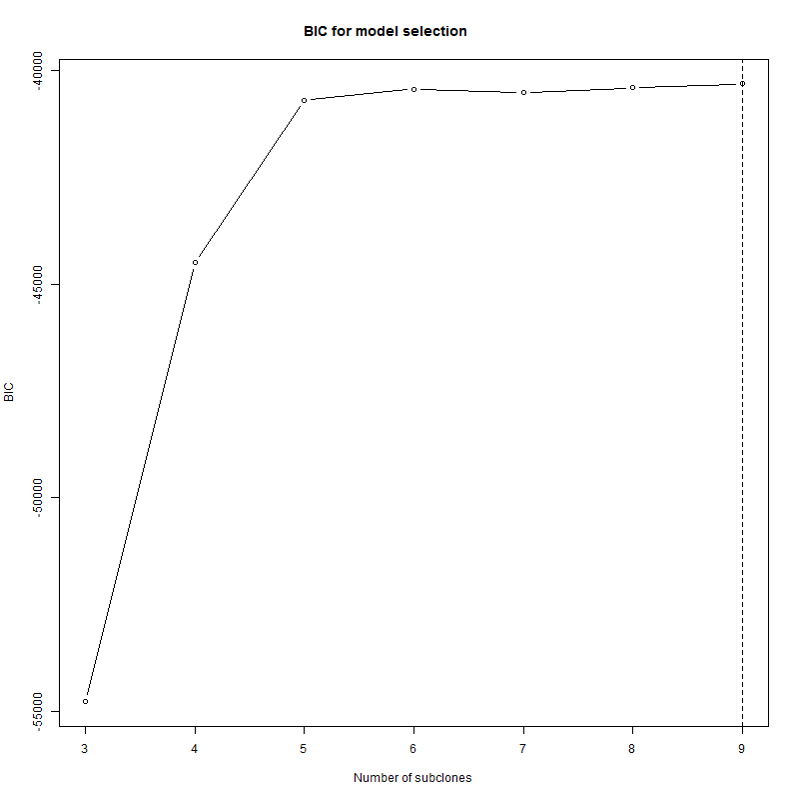
\includegraphics[width=0.7\linewidth,keepaspectratio]{images/240/bic}
	\caption[BIC scores of subclonal models with 3--9 clonal populations.]{BIC score of subclonal models with 3--9 clonal populations. Models with 3 to 9 clonal populations were tested by Canopy. A five-population model was selected (BIC = -40,684.12), as higher-complexity models did not yield substantially higher BIC (maximal BIC = -40,301.74 with 9 clonal populations). Note that germline is considered a clonal population by Canopy, therefore the selected model contains four tumor subclones.}
	\label{fig:240:bic}
\end{figure}
Canopy computes a Bayesian Information Criterion \cite{schwarz1978} (BIC) score for each potential number of subclones, which was used to determine the number of subclones that best represents the data. A 4-clone model was selected since models with additional subclones only yielded marginal increases in BIC (Figure~\ref{fig:240:bic}). Note that Canopy estimates its normal cell fractions based on variant fractions and CNV data, and reported purities can differ from pathologist estimates, likely because different sections of the tumor blocks were sequenced than were reviewed by the pathologist (Supplemental File~S\thechapter{}.5).

\subsubsection[Post hoc mutation assignment]{\textit{Post hoc} mutation assignment}
\label{ssec:240:tree_assignment}
Afterwards, the remaining somatic SNVs (not used for Canopy tree building) and indels were retroactively assigned to the resulting tree using a maximal likelihood model. From Canopy, we have a phylogenetic tree $G = (V, E)$, in which $v_1$ corresponds to the patient's germline and other vertices correspond to tumor subclones. Define $N$ as the number of tumor samples. For an arbitrary somatic mutation $m$, define $\vec{r} \in \mathbb{Z}^N$ as the number of alternate-supporting reads for $m$ in each sample, $\vec{x} \in \mathbb{Z}^N$ as the coverage of the variant position in each sample, and $\vec{p} \in \mathbb{R}^N$, a vector of expected variant fractions in each sample (derived from the tree as shown below). Given known $\vec{x}$ and $\vec{p}$, and modeling alternative read depth as jointly binomial across tumor samples, the probability and log-likelihood that $m$ is within an edge $e \in E$ can be computed as follows:
\begin{subequations}
    \begin{equation}
        P(\vec{r} | \vec{x}, \vec{p}) = \prod_{i=1}^{N} \dbinom{x_i}{r_i} p_i^{r_i} (1 - p_i)^{(x_i - r_i)}
    \end{equation}
    \begin{align}
        \mathcal{L}(m \in e) &= \ln\left(P(\vec{r} | \vec{x}, \vec{p})\right) \nonumber \\
        &= \sum_{i=1}^N \left( \sum_{j=r_i + 1}^{x_i} \ln(j) - \sum_{j=1}^{x_i - r_i} \ln(j) + r_i \ln(p_i) + (x_i - r_i) \ln(1 - p_i) \right)
    \end{align}
\end{subequations}

To compute $\vec{p}$, we utilize the phylogenic tree and clonal fractions reported by Canopy, along with its per-subclone major and minor copy number estimates. We construct a matrix $\mathbf{T} \in \{0, 1\}^{|E| \times |V|}$ as follows:
\begin{equation}
    T_{e, v} = \begin{cases}
        1 & \text{if the path from } v_1 \text{ to vertex } v \text{ contains edge } e \\
        0 & \text{otherwise}
    \end{cases} \qquad e \in E, v \in V
\end{equation}

From CNV calling, we have $T$, the number of CNV regions. We also have from Canopy the clonal matrix $\mathbf{P} \in \mathbb{R}^{|V| \times N}$, in which each column corresponds to the proportions of the respective subclone (or germline) in each tumor sample, $\tilde{\mathbf{C}}^M \in \mathbb{Z}^{T \times |V|}$ as the per-subclone major copy number matrix, and $\tilde{\mathbf{C}}^m \in \mathbb{Z}^{T \times |V|}$ as the per-subclone minor copy number matrix. Any zero values within each column of $\mathbf{P}$ were set to $0.0005$, and remaining entries reduced equally to maintain the constraint that each column sums to 1. This is first used to compute $\mathbf{A} \in \mathbb{R}^{T \times N}$, the total copy number of each CNV-affected region in each sample (independent of any specific mutation), as follows:
\begin{equation}
    \mathbf{A} = (\tilde{\mathbf{C}}^M + \tilde{\mathbf{C}}^m)\mathbf{P}
\end{equation}

Next, assume without loss of generality that mutation $m$ is within edge $e$. If $m$ is within a CNV $t$, we know from Canopy the edge $y \in E$ that contains $t$. We can calculate the copy number of $m$ in each subclone, $\vec{b} \in \mathbb{Z}^{|V|}$, as follows:
\begin{subequations}
    \begin{equation}
        \mathbf{C} = \begin{cases}
            \tilde{\mathbf{C}}_{t*}^M & m \text{ is on major allele of CNV } t \text{, and } y \text{ is further from } v_1 \text{ than } e \\
            \tilde{\mathbf{C}}_{t*}^m & m \text{ is on minor allele of CNV } t \text{, and } y \text{ is further from } v_1 \text{ than } e \\
            \{1\}^K & m \text{ is not within any CNV, or } e \text{ is further from } v_1 \text{ than } y
        \end{cases}
    \end{equation}
    \begin{equation}
        \vec{b} = (\mathbf{T}_{e*} \circ \mathbf{C})\mtpose
    \end{equation}
\end{subequations}
where $\circ$ is the Hadamard product of matrices. This permits calculation of the expected copy number of $m$ in each sample $\vec{s} \in \mathbb{R}^N$, provided that $m \in$ an edge $e$ and $m$ is on a major or minor allele, as follows:
\begin{equation}
    \vec{s} = \mathbf{P}\mtpose \vec{b}
\end{equation}
Computation of $\vec{p}$ for mutation $m$ is now straightforward:
\begin{equation*}
    \vec{a} = \begin{cases}
        \mathbf{A}_{t*}\mtpose & m \text{ is within CNV } t \\
        \{2\}^N & m \text{ is not within an CNV, and is on an autosome or chrX in a female} \\
        \{1\}^N & m \text{ is on chrX or chrY in a male}
    \end{cases}
\end{equation*}
\begin{equation}
    p_i = \frac{s_i}{a_i} \qquad i = 1 \twodots N
\end{equation}

To perform the assignment of mutation $m$, $\mathcal{L}(m \in e)$ is computed for all edges $e \in E$. If $m$ is within a CNV region and the candidate edge is before the CNV, its possibilities of being on the major or minor allele are both considered. If the candidate edge is after the CNV, only the possibility of it occurring on one copy of the allele is considered, utilizing the simplifying assumptions (also made by Canopy) that each somatic mutation occurs only once and no back-mutations occur. If the candidate edge contains the CNV, all three above possibilities (major\slash{}minor\slash{}after) must be considered. To avoid numerical errors, if $p_i = 0$ and $r_i \neq 0$ for a candidate assignment in any sample, that candidate assignment is discarded. The edge with highest log-likelihood is selected, with ties (such as can occur with deletions or on a different edge than a CNV) broken in favor of the edge furthest from the root node. This approach was implemented and run using Python 2.7.1, using scipy \cite{2020SciPy-NMeth} 0.10.1.

\subsubsection{Mutational ordering}
\label{ssec:240:mutational_ordering}
Mutations within each branch of the tree were temporally ordered using a Bradley-Terry model \cite{terry52}. Given a phylogenetic tree $G = (V, E)$ from Canopy and \textit{post hoc} tree assignment, we have a set of mutations $M_e$ for each edge $e \in E$. Define $\vaf_i(m)$ as the variant fraction (VF) of mutation $m$ in tumor sample $i \in 1..S$, where $S$ is the set of tumor samples used to build $G$.

We regard each pair of variants $m_1, m_2 \in M_e$ in each tree edge and sample as a contest, with the \emph{score} of $m_1$ vs.\ $m_2$ in sample $i$ as follows:
\begin{equation}
	w_i(v_1, v_2) = 
	\begin{cases}
		1 & \vaf_i(m_1) > \vaf_i(m_2) \\
		0 & \vaf_i(m_1) < \vaf_i(m_2) \\
		0.5 & \vaf_i(m_1) = \vaf_i(m_2)
	\end{cases}
\end{equation}
Summing all pairwise scores from all samples yields the wins matrix $\mathbf{V} \in \mathbb{R}^{|M_e| \times |M_e|}$:
\begin{equation}
	V_{jk} = \begin{cases} \sum_{i=1}^S w_i(m_j, m_k) & j \ne k \\ 0 & j = k \end{cases} \qquad j, k \in 1..|M_e|
\end{equation}

The Bradley-Terry model yields \emph{abilities} $\pi_m$ for each mutation, such that:
\begin{equation}
	P(m_1 \text{ occurred before } m_2) = \frac{\pi_1}{\pi_1 + \pi_2}
\end{equation}
where $\pi_1$ and $\pi_2$ are the abilities of mutations $m_1$ and $m_2$. The maximum \textit{a priori} estimate of abilities \cite{btbayesian} was computed using the R package \texttt{BradleyTerryScalable} \cite{btscalable} with $a = 1.1$. Note that ability scores denote confidence in ordering, not the time intervals between acquisition of mutations. This analysis was performed independently for each edge of the clonal phylogeny tree, utilizing both mutations supplied to Canopy and those retroactively assigned to the tree.

\subsection{Droplet digital PCR and analysis}
Isolated genomic DNA was amplified using a custom designed probe for the \textit{FGFR2} N549H point mutation (PrimePCR ddPCR Mutation Assay, Bio-Rad\textsuperscript\textregistered{}) and the ddPCR Supermix for Probes (Bio-Rad). The reaction mixture consisted of 250 ng of DNA template (8~\textmu{}L), 10~\textmu{}L of ddPCR Supermix for Probes (Bio-Rad) and 2~\textmu{}L of the primer/probe mixture. Droplets were generated using the QX200 Droplet Generator (Bio-Rad) and then transferred to a 96-well plate (Eppendorf\textsuperscript\textregistered{}) for PCR amplification with the following conditions: 5 minutes at 95~\textdegree{}C, 40 cycles of 94~\textdegree{}C for 30 seconds, 55~\textdegree{}C for 1 minute followed by 98~\textdegree{}C for 10 minutes (ramp rate 2~\textdegree{}C/second). Droplets were analyzed with the QX200 Droplet Reader (Bio-Rad) for fluorescent measurement of FAM and HEX probes. Gating was performed based on positive and negative controls, and mutant populations were identified. All reactions were run in duplicate. The ddPCR data were analyzed with QuantaSoft analysis software (Bio-Rad) to obtain fractional abundance of the mutant DNA alleles in the wild-type (WT)/normal background.

\subsection{cDNA plasmid generation, lentivirus production and transduction}
\begin{figure}[htp]
	\centering
	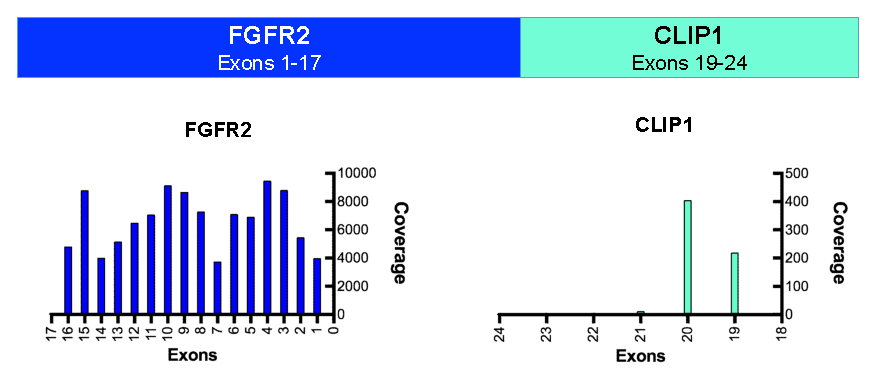
\includegraphics[width=0.8\linewidth,keepaspectratio]{images/240/fusion_coverage}
	\caption[RNA-seq coverage of novel FGFR2-CLIP1 fusion.]{RNA-seq coverage of novel FGFR2-CLIP1 fusion. A novel fusion containing exons 1--17 of \textit{FGFR2} and exons 19--24 of \textit{CLIP1} was detected in a patient with cholangiocarcinoma.}
	\label{fig:240:fusion_coverage}
\end{figure}
The \textit{FGFR2-CLIP1} fusion was produced and cloned into the pLVX-IRES-Puro vector (Clontech) by GenScript\textsuperscript\textregistered{}, containing exons 1--17 of \textit{FGFR2} and exons 19--24 of \textit{CLIP1} (Figure~\ref{fig:240:fusion_coverage}). Using site directed mutagenesis, the \textit{FGFR2} N549H mutation was introduced into the fusion by GenScript. NIH3T3 cells were stably transduced with either empty, \textit{FGFR2-CLIP1} or \textit{FGFR2-CLIP1} N549H lentiviral vectors. Cells were selected in puromycin (1~\textmu{}g/mL; Sigma-Aldrich\textsuperscript\textregistered{}) for 72 hours prior to their use in downstream experiments.

\subsection{RNA isolation, RT-PCR and Sanger sequencing}
\begin{table}[H]
    {\small
	\begin{center}
		\begin{tabular}{cccc}
			 & & & \textbf{Product} \\
			\textbf{Target} & \textbf{Forward} & \textbf{Reverse} & \textbf{Size (bp)} \\
			\hline
			FGFR2-CLIP1 & 5'--\texttt{CAGAGACCAACGTTCAAGCA}--3' & 5'--\texttt{CGGCATCCTTTTCTGTGAGT}--3' & 214 \\
			N549H & 5'--\texttt{GTGGCCGTGAAGATGTTGAA}--3' & 5'--\texttt{AGGTATTCTCGGAGGTTGCC}--3' & 188
		\end{tabular}
	\end{center}}
	\vspace{-0.3cm}
	\caption[Primer sequences.]{Primer sequences used for PCR and Sanger sequencing to confirm the presence of either the fusion or the mutation.}
	\label{table:240:primer_seqs}
\end{table}
RNA was isolated from cell lines, and cDNA was synthesized using The Quick-RNA Mini Prep Kit (Zymo Research\textsuperscript\texttrademark{}) and the iScript cDNA Synthesis Kit (Bio-Rad), respectively. cDNA was subsequently PCR amplified with \textit{FGFR2-CLIP1} and \textit{FGFR2} N549H fusion specific primers (IDT)\@. Primer sequences are listed in Table~\ref{table:240:primer_seqs}. The Invitrogen PureLink Quick PCR Purification Kit (Thermo Fisher) was used to purify amplified PCR product and samples were then Sanger sequenced (The Ohio State University Comprehensive Cancer Center Genomics Shared Resource, Columbus, OH).

\subsection{Cell culture}
NIH3T3 and HEK293T cell lines were purchased from American Type Culture Collection (ATCC\textsuperscript\textregistered{}) and cultured in a humidified incubator at 37~\textdegree{}C and 5\%~CO\textsubscript{2}. Cells were cultured according to ATCC recommended protocols. All cell lines were routinely subjected to short tandem repeat profiling to confirm identities and \textit{Mycoplasma} testing using the e-Myco Plus Mycoplasma PCR Detection Kit (Bulldog Bio\textsuperscript\texttrademark{}).

\subsection{Western blotting}
Western blot assays were carried out using established protocols and probed with the following antibodies: phospho-Akt (Ser473) 1:1000 (Cell Signaling Technology\textsuperscript\textregistered{} 9271), Total Akt 1:1000 (Cell Signaling 9272), phospho-MEK1/2 1:5000 (Cell Signaling 9154), Total MEK1/2 1:5000 (Cell Signaling 9122), p44/42 MAPK (Erk1/2) 1:5000 (Cell Signaling 9101), Total MAPK 1:5000 (Cell Signaling 9102), phospho-FGF Receptor (Tyr653/654) 1:500 (Cell Signaling 3471), FGF Receptor 2 (D4L2V) 1:500 (Cell Signaling 23328),  phospho-PLC$\gamma$1 (Tyr783) 1:1000 (Cell Signaling 14008), PLC$\gamma$1 (D9H10) 1:1000 (Cell Signaling 5690), phospho-FRS2\nobreakdash-$\alpha$ (Tyr196) 1:1000 (Cell Signaling 3864), FRS2 1:1000 (Abcam\textsuperscript\textregistered{} 10425), phospho-PI3 Kinase p85 (Tyr458)/p55 (Tyr199) 1:1000 (Cell Signaling 4228), PI3 Kinase p85 (19H8) 1:1000 (Cell Signaling 4257), $\beta$-actin 1:10000 (Cell Signaling 4967).

\subsection{Drug sensitivity assays}
NIH3T3 Empty, \textit{FGFR2-CLIP1}, and \textit{FGFR2-CLIP1} N549H cells were plated at a density of 10,000 cells per well in 96-well plates. Cells were treated for 72 hours with either INCB054828 (Incyte\textsuperscript\textregistered{}), BGJ398 (Cayman Chemical\textsuperscript\textregistered{}), JNJ-42756493 (Cayman Chemical), AZD-4547 (Cayman Chemical), ponatinib (Cayman Chemical), or dovitinib (Cayman Chemical) ranging from 0.01 to 5000~nM\@. Quantification of viable cells was assessed using an MTS/PMS colorimetric assay. IC\textsubscript{50} values were calculated in Prism (GraphPad) using a 4-parameter dose-response model.

\section{Results}
\subsection{Clinical course}

\begin{figure}[htp]
    \centering
    \begin{subfigure}{0.8\textwidth}
        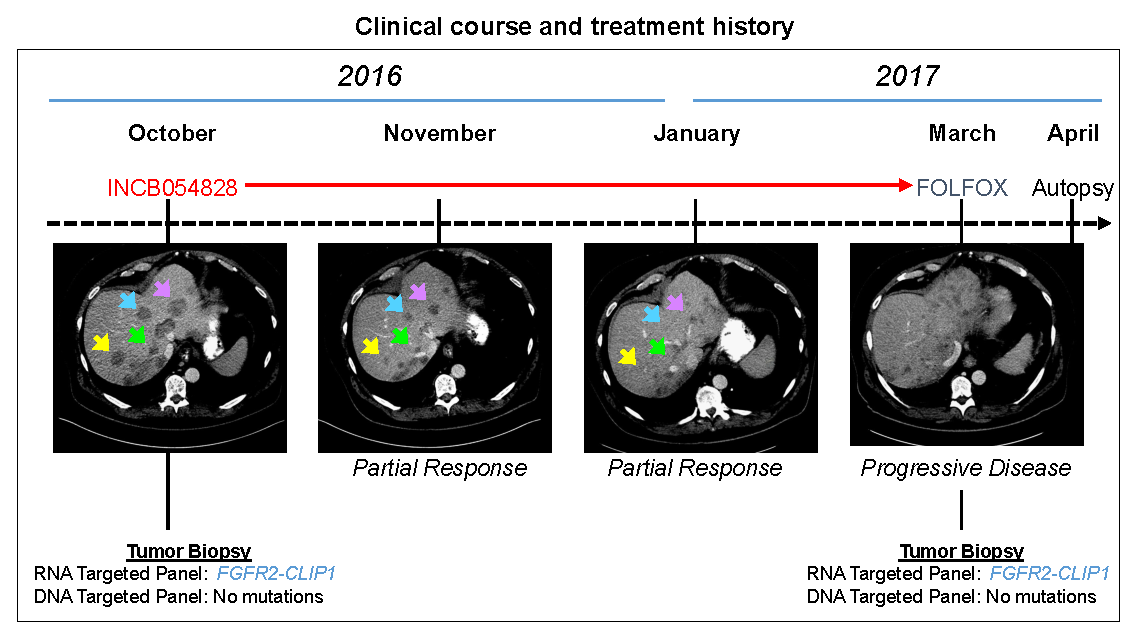
\includegraphics[width=\textwidth,keepaspectratio]{images/240/clinical_course}
        \caption{}\label{fig:240:clinical_course}
    \end{subfigure}\par
    \begin{subfigure}{0.8\textwidth}
        
\includegraphics[width=\textwidth,keepaspectratio]{images/240/recist}
        \caption{}\label{fig:240:recist}
    \end{subfigure}\par
    \begin{subfigure}{0.8\textwidth}
        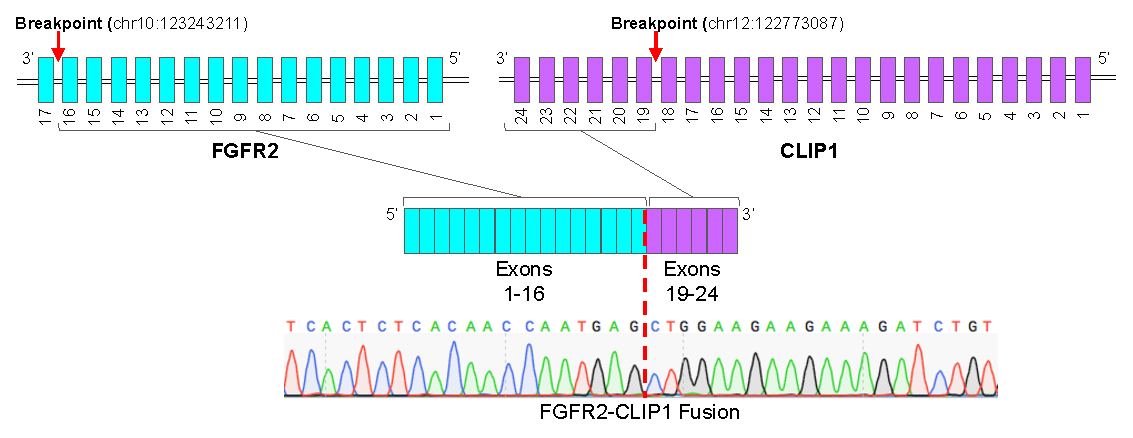
\includegraphics[width=\textwidth,keepaspectratio]{images/240/fusion_schematic}
        \caption{}\label{fig:240:fusion_schematic}
    \end{subfigure}
    \vspace{-0.2cm}
    \caption[Description of a cholangiocarcinoma patient harboring an FGFR2-CLIP1 fusion.]{Description of a patient with metastatic cholangiocarcinoma harboring an \textit{FGFR2-CLIP1} fusion. (\subref{fig:240:clinical_course}) Clinical course of this patient with selected CT scans. (\subref{fig:240:recist}) Table summarizing two target lesions (posterior hepatic dome lesion and left hepatic lobe lesion) that were tracked throughout the treatment course and had a 24.8\% and 46.5\% reduction from baseline after cycles 3 and 6, respectively. (\subref{fig:240:fusion_schematic}) Schematic of the \textit{FGFR2-CLIP1} fusion involving exons 1--16 of \textit{FGFR2} and exons 19--24 of \textit{CLIP1}. Chromatogram traces from Sanger sequencing of the tumor biopsy confirmed the presence of the fusion. Red dashed line indicates breakpoint within sequence.}
    \label{fig:240:clinical_desc}
\end{figure}
A 59-year old male presented clinically with abdominal pain and fullness in the fall of 2015 (Figure~\ref{fig:240:clinical_course}). Abdominal CT and MRI scans revealed two small but suspicious appearing lesions in the liver. He underwent biopsy of one liver lesion and pathology demonstrated poorly differentiated adenocarcinoma with focal neuroendocrine differentiation (CK7\textsuperscript{+}, CDX2\textsuperscript{+}, synaptophysin\slash{}chromogranin\textsuperscript{+}, CK20\textsuperscript{-}, TTF1\textsuperscript{-}, napsin\textsuperscript{-}) consistent with pancreatic or biliary origin. A PET-CT scan showed localized cancer in the right hepatic lobe, and he subsequently underwent surgical resection with clear margins and no lymph node involvement. Surgical pathology confirmed intrahepatic cholangiocarcinoma, which was staged as T2aN0. He received no adjuvant therapy post-surgery. Five months later, in April 2016, surveillance MRI showed emergence of new hepatic tumors, prompting palliative treatment with gemcitabine and cisplatin (Gem/Cis). Gemcitabine (1000~mg/m\textsuperscript{2}) and cisplatin (25/m\textsuperscript{2}) were given on D1 and D8 of a 21-day cycle.  In June 2016, after two cycles of chemotherapy, CT scans revealed numerous hypodense lesions consistent with worsening of hepatic metastatic disease and Gem/Cis was stopped.  At this time, he underwent a repeat tumor biopsy and RNA profiling of his cancer using an NGS assay, OSU-SpARKFuse \cite{reeser2017}, which revealed a novel gene fusion involving \textit{FGFR2} (exons 1--16) and \textit{CLIP1} (exons 19--24) (Figure~\ref{fig:240:fusion_coverage}). The presence of the fusion was confirmed by reverse transcription PCR and Sanger sequencing with primers designed to flank the breakpoint (Figure~\ref{fig:240:fusion_schematic}). CLIP1 is a CAP-Gly domain-containing linker protein 1 that has been shown to regulate the microtubule cytoskeleton. Based on the presence of this novel FGFR2-CLIP1 fusion in his cancer, at the beginning of October the patient enrolled in a Phase I/II clinical trial (NCT02393248) evaluating the safety and tolerability of an oral pan-FGFR inhibitor, INCB054828. He received 13.5~mg once daily for days 1--14 per 21-day cycle. Disease assessment after cycles 3 (November) and 6 (January) showed robust partial response by RECIST criteria, consistent with this novel FGFR2 fusion being a driver of his metastatic cancer (Figure~\ref{fig:240:clinical_course}). As part of the study, two target lesions (posterior hepatic dome lesion and left hepatic lobe lesion) were tracked throughout the treatment course and had a 24.8\% and 46.5\% reduction from baseline after cycles 3 and 6, respectively (Figure~\ref{fig:240:recist}). Prior to starting cycle 8, he was admitted to the hospital with significant weight loss and elevated liver function tests (LFTs) suggesting disease progression. After a total of 5.5 months (7 cycles) on INCB054828, CT scans showed a 41.3\% increase in size of the two target lesions confirming progressive disease. At this time, he underwent a repeat post-progression tumor biopsy which confirmed the continued presence of the FGFR2-CLIP1 fusion (Figure~\ref{fig:240:clinical_course}). One month after receiving the last dose of INCB045828, second-line chemotherapy (FOLFOX) was initiated. He received a single dose of oxaliplatin (190~mg) and fluorouracil (3975~mg). However, he passed away 11 days after receiving this single dose of FOLFOX due to liver failure. Prior to passing, he consented to our body donation study for patients with advanced cancer.
\subsection{Research autopsy reveals clonal heterogeneity in cholangiocarcinoma}
\label{ssec:240:autopsy_results}

\begin{figure}[htp]
    \centering
    \begin{subfigure}{0.6\textwidth}
        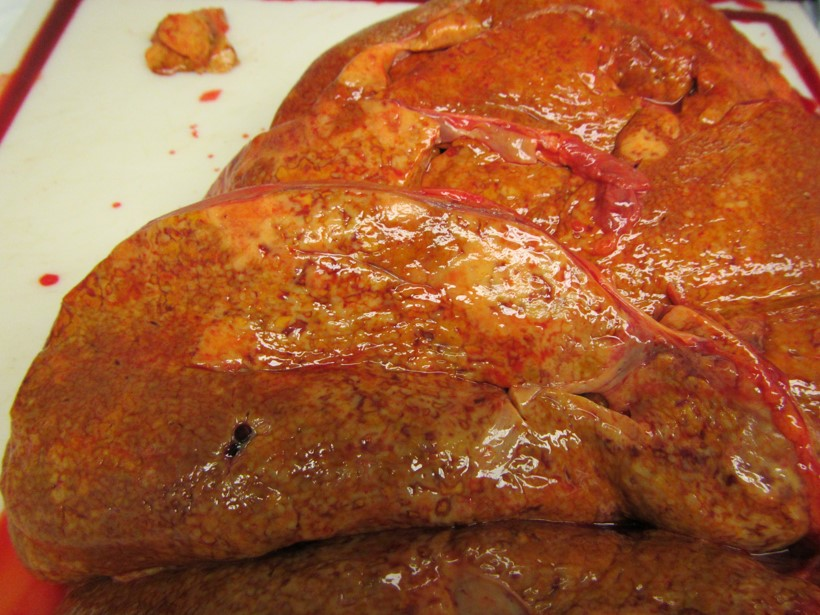
\includegraphics[width=\textwidth,keepaspectratio]{images/240/autopsy_gross}
        \caption{}\label{fig:240:autopsy_gross}
    \end{subfigure}\par
    \begin{subfigure}{0.7\textwidth}
        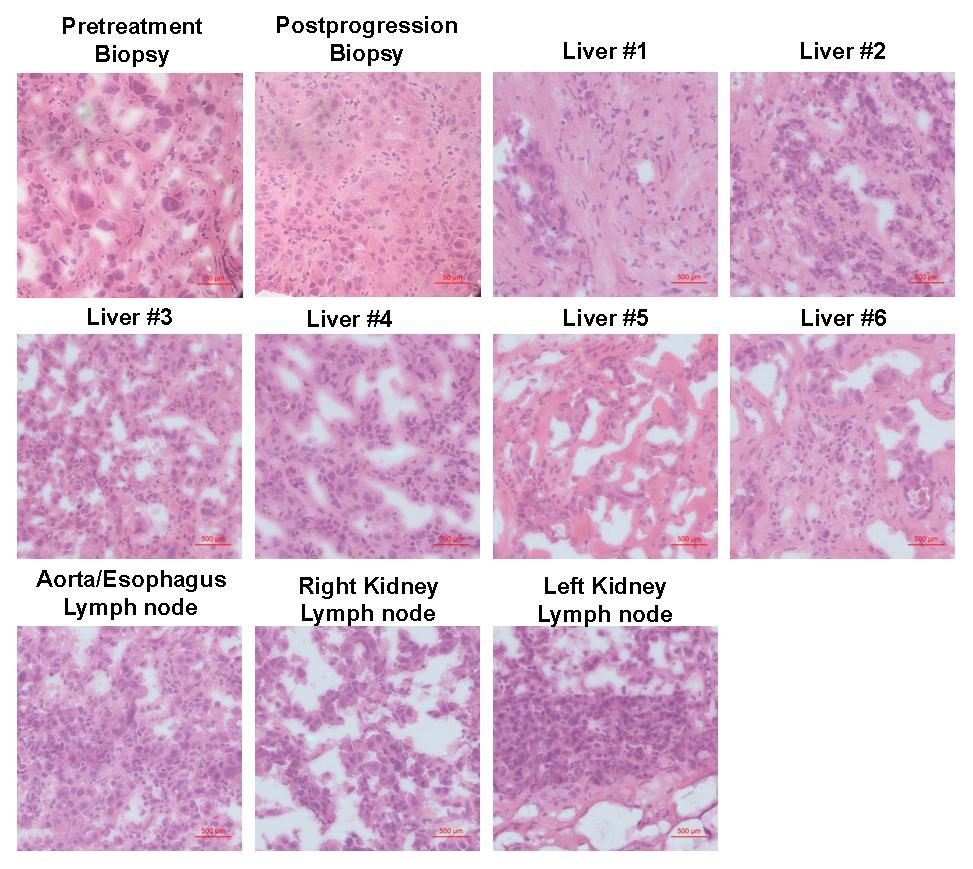
\includegraphics[width=\textwidth,keepaspectratio]{images/240/histo}
        \caption{}\label{fig:240:histo}
    \end{subfigure}
    \caption[Research autopsy of a cholangiocarcinoma patient with an FGFR2-CLIP1 fusion.]{Research autopsy of a cholangiocarcinoma patient with an FGFR2-CLIP1 fusion. (\subref{fig:240:autopsy_gross}) Gross image of the liver at the time of autopsy. (\subref{fig:240:histo}) Hematoxylin and eosin (H\&E) stains of representative slides taken from each tumor sample demonstrating abundant malignant cells.}
    \label{fig:240:autopsy}
\end{figure}
Upon death of this patient, a research autopsy was performed eight hours post-mortem. Gross examination revealed metastatic tumors involving the liver, omentum, and abdominal and retroperitoneal lymph nodes. Twenty-four liver tumor samples and 5 separate lymph nodes were procured at the time of autopsy. While we attempted to sample distinct liver tumors, the patient's liver was predominately cancerous with limited grossly normal liver tissue present (Figure~\ref{fig:240:autopsy_gross}). Samples used for subsequent analysis had at least 40\% tumor content as determined by a board-certified pathologist (Figure~\ref{fig:240:histo}).

% Table generated by Excel2LaTeX from sheet 'Sheet1'
\begin{table}[htbp]
    \centering
    {\small
    \begin{tabular}{cccccc}
         & \textbf{\% Tumor} & \textbf{Average} & \textbf{Number} & \textbf{Number} & \textbf{TMB} \\
        \textbf{Sample} & \textbf{Cells} & \textbf{Coverage (X)} & \textbf{of SNVs} & \textbf{of Indels} & \textbf{(Muts/Mb)} \\
        \hline
        Pretreatment & 40\%  & 181.19 & 44    & 6     & 1.3 \\
        Postprogression & 50\%  & 222.90 & 79    & 8     & 2.2 \\
        Liver \#1 & 50\%  & 252.23 & 101   & 13    & 2.9 \\
        Liver \#2 & 50\%  & 238.64 & 87    & 10    & 2.5 \\
        Liver \#3 & 40\%  & 229.92 & 99    & 10    & 2.8 \\
        Liver \#4 & 50\%  & 263.33 & 93    & 5     & 2.5 \\
        Liver \#5 & 40\%  & 230.61 & 56    & 9     & 1.7 \\
        Liver \#6 & 50\%  & 236.28 & 76    & 7     & 2.1 \\
        Aorta/esophagus LN & 50\%  & 236.78 & 88    & 6     & 2.4 \\
        Right Kidney LN & 40\%  & 227.86 & 73    & 11    & 2.2 \\
        Left Kidney LN & 60\%  & 216.78 & 89    & 9     & 2.5 \\
    \end{tabular}}
    \caption[Tumor content and WES metrics for each tumor sample sequenced.]{Summary of estimated tumor content and whole exome sequencing metrics within each sample. SNV: single nucleotide variant. TMB: tumor mutational burden. LN: lymph node.}
    \label{table:240:wes}
\end{table}
In total, a normal blood control and 11 tumor samples (1 pre-treatment tumor biopsy, 1 post-progression tumor biopsy, and 9 autopsy tumor samples) were chosen for further analysis (Table~\ref{table:240:wes}). Sanger sequencing confirmed that the FGFR2-CLIP1 fusion was present in each tumor sample (data not shown). DNA from these tumors were subjected to whole exome sequencing, yielding 231\texttimes{} average target coverage and revealed a total of 979 somatic variants across all tumors (292 unique somatic variants) \cite{samorodnitsky2015_hyb_amplicon}. 242 of these mutations were unique to the post-progression and autopsy samples (Supplemental File~S\thechapter{}.6). The tumor mutational burden (TMB) of samples ranged from 1.3~muts/Mb in the pre-treatment biopsy to 2.9~muts/Mb in liver sample \#1, consistent with previous studies indicating low TMB in cholangiocarcinoma \cite{chalmers2017,nakamura2015}. All tumor samples were determined to be microsatellite stable (MSS) through analysis of 2,539 loci by MANTIS \cite{kautto17}. Mutational signatures 16 and 19 were common across tumor samples. Signature 16 has been found in liver cancer and signature 19 has been found in pilocytic astrocytoma, however their etiologies are unknown \cite{cosmic_ms}.

\begin{figure}[htp]
	\centering
	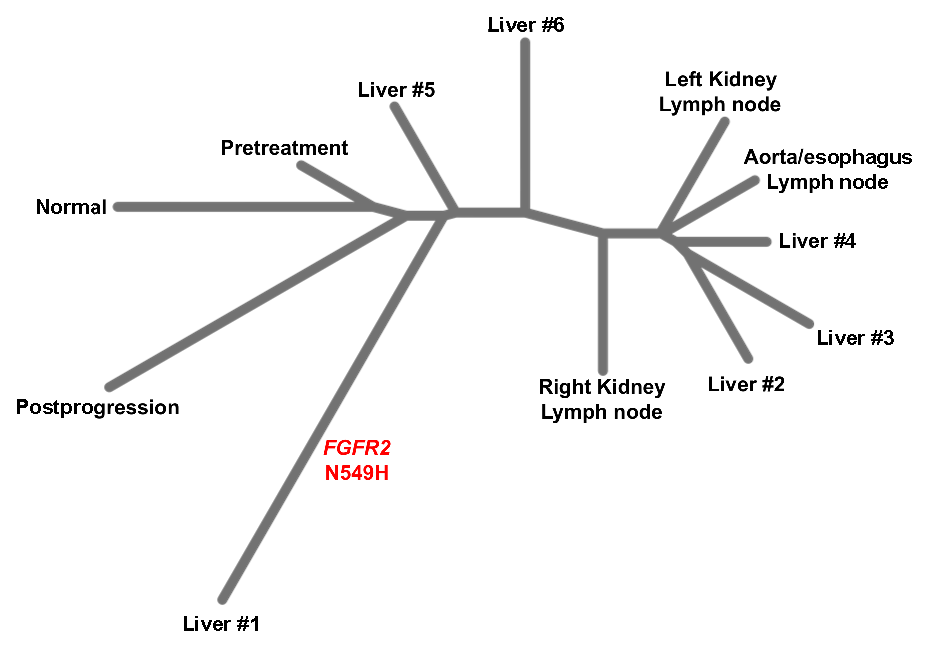
\includegraphics[width=0.8\linewidth,keepaspectratio]{images/240/nj_tree}
	\caption[Neighbor joining tree over 11 cholangiocarcinoma tumor samples.]{Neighbor joining tree over 11 cholangiocarcinoma tumor samples. The tree was calculated over sets of somatic SNVs in each tumor sample, with normal defined as the empty set.}
	\label{fig:240:nj_tree}
\end{figure}
The somatic single nucleotide variants (SNVs) called in each tumor sample were subsequently used to build a phylogenetic tree of tumor samples via the neighbor joining (NJ) method \cite{saitou1987} (Figure~\ref{fig:240:nj_tree}). As expected, the pre-treatment sample branched most closely to the normal cells; the two samples are separated by a relatively short genetic distance of 33.2 indicating a high degree of genetic similarity. The post-progression sample had the next closest genetic similarity to the normal, with a genetic distance of 37.6. The liver \#1 sample was the most genetically unique tumor sample with a genetic distance of 100.1 from the normal. Liver samples \#2, 3, and 4 were clustered with the aorta/esophagus lymph node and left kidney lymph node.

\begin{figure}[htbp]
	\centering
	\begin{subfigure}{0.4\textwidth}
		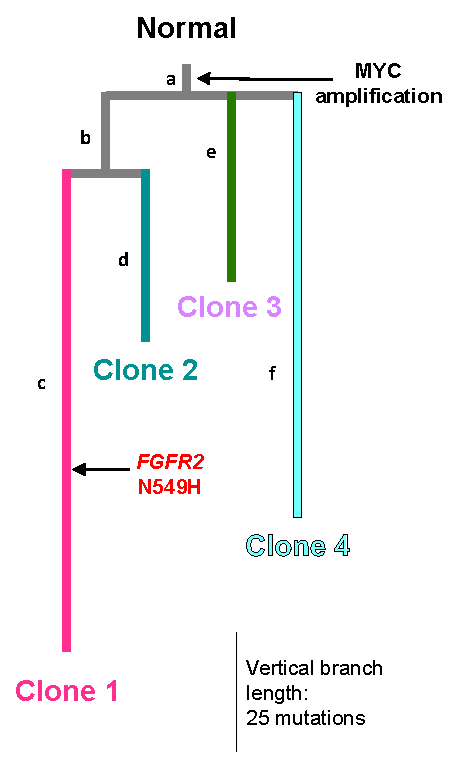
\includegraphics[width=\textwidth,keepaspectratio]{images/240/canopy_tree}
		\caption{}\label{fig:240:canopy_tree}
	\end{subfigure}%
	\hfill%
	\begin{subfigure}{0.55\textwidth}
		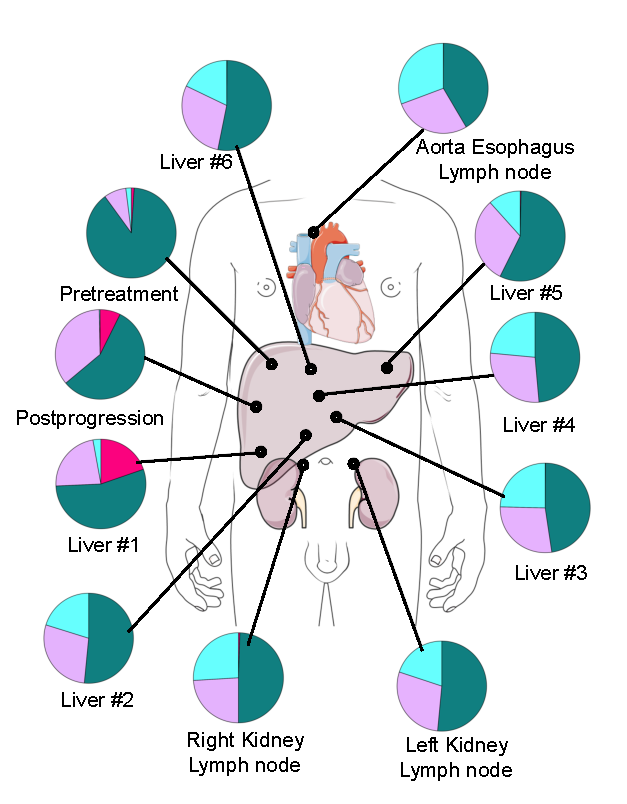
\includegraphics[width=\textwidth,keepaspectratio]{images/240/canopy_clonal_fracs}
		\caption{}\label{fig:240:canopy_clonal_fracs}
	\end{subfigure}
	\caption[Subclonal inference from Canopy.]{Subclonal inference from Canopy. Colors in (\subref{fig:240:canopy_tree}) correspond to subclones in (\subref{fig:240:canopy_clonal_fracs}). Letters identify branches of the tree. (\subref{fig:240:canopy_tree}): Phylogenetic tree assessment with Canopy revealed four major clonal populations of cells. Each subclone is characterized by a group of mutations. MYC gain was truncal to all subclones. Clone 1 (pink) contained a unique \textit{FGFR2} N549H point mutation. Vertical distance corresponds to increased number of somatic mutations (SNVs and indels). (\subref{fig:240:canopy_clonal_fracs}) Prevalence of four tumor subclones within tumor samples.}
	\label{fig:240:canopy_results}
\end{figure}
We next utilized Canopy \cite{canopy} to computationally identify and characterize tumor subclones using both synonymous and nonsynonymous somatic SNVs, CNVs, and indels (Figure~\ref{fig:240:canopy_results}). With this analysis, we identified 4 tumor subclones across the 11 samples, with each subclone characterized by a unique group of genomic alterations (Figure~\ref{fig:240:canopy_tree}, Supplemental Files~S\thechapter{}.5, S\thechapter{}.7--8). Clones 2 (teal) and 3 (purple) were shared among all samples (Figure~\ref{fig:240:canopy_clonal_fracs}). Clone 4 (cyan) was seen in all except one autopsy sample (liver \#1) and was not present in the pre-treatment or post-treatment samples. 89\% of the tumor cells in the pre-treatment sample were estimated to be from clone 2, versus approximately 40--60\% of the other samples. Clone 1 (pink) was primarily found in liver \#1 (20\%) and at low frequency in the post-treatment sample (7\%). This is consistent with the NJ tree, as the relatively large number of mutations unique to clone 1 accounts for the distance of liver \#1 and the post-progression samples from all other samples.

\begin{table}[htp]
    \centering
    \begin{tabular}{cc}
        \textbf{Sample} & \textbf{\% Mutant} \\
        \hline
        Negative Control & 0\% \\
        Positive Control & 95\% \\
        Pretreatment & 0\% \\
        Postprogression & 0\% \\
        Liver \#1 & 17.60\% \\
        Liver \#2 & 0.30\% \\
        Liver \#3 & 0.14\% \\
        Liver \#4 & 0\% \\
        Liver \#5 & 0\% \\
        Liver \#6 & 0\% \\
        Aorta/esophagus Lymph node & 0\% \\
        Right Kidney Lymph node & 0\% \\
        Left Kidney Lymph node & 0\%
    \end{tabular}
    \caption[ddPCR for FGFR2 N549H mutation.]{Droplet digital PCR (ddPCR) results for percentage of \textit{FGFR2} N549H mutant present in samples.}
    \label{table:240:ddpcr}
\end{table}
Of the 292 distinct mutations (SNVs and indels) identified among these samples, only seven were truncal (\textit{i.e.}\ common to all four subclones). Most notable among the truncal events (branch \textbf{\textit{a}}) was a 21.9 Mb gain in chromosome 8q (chr8:124448804--146364022), containing \textit{MYC} among other genes. Although Canopy did not identify non-truncal mutations shared by clones 3 and 4, \textit{post hoc} assignment was permitted to assign mutations to a hypothetical unique common ancestor. No such mutations were assigned, suggesting that clones 3 and 4 diverged relatively early in the tumor's evolution. Of clinical interest, whole exome sequencing revealed an FGFR2 kinase domain mutation, \textit{FGFR2} N549H in a single liver tumor, liver \#1 (Figure~\ref{fig:240:nj_tree}). The \textit{FGFR2} N549H mutation occurs in the kinase hinge and has been shown to disengage the molecular breaker resulting in ligand-independent constitutive activation of the FGFR2 kinase \cite{chen2007}. The \textit{FGFR2} N549H mutation was assigned uniquely to clone 1, which was the most genetically distinct subclone compared to the patient's normal blood DNA (Figure~\ref{fig:240:canopy_tree}). Although clone 1 was predicted to be present at low frequency in the post-progression sample, \textit{FGFR2} N549H was not detected in this sample. ddPCR of all samples confirmed that the \textit{FGFR2} N549H mutation was unique to liver \#1 (Table~\ref{table:240:ddpcr}). Of the 111 mutations unique to clone 1, this mutation was estimated to be the 63\textsuperscript{rd} to occur. This led us to hypothesize that the \textit{FGFR2} N549H kinase domain mutation may have been partially responsible for driving resistance to INCB054828 in this patient, occurring along an existing clonal lineage. Driver mutation prediction with CHASM \cite{carter2009} predicted only \textit{FGFR2} N549H to be a statistically likely driver (defined as FDR-corrected $P \le 0.05$ (Supplemental File~S\thechapter{}.9).

\subsection[In vitro characterization of acquired mutations in FGFR2-CLIP1 and resistance to INCB054828]{\textit{In vitro} characterization of acquired mutations in \textit{FGFR2-CLIP1} and resistance to INCB054828}
\begin{figure}[htbp]
    \begin{minipage}[t]{0.22\textwidth}
        \vspace{0pt}
        \begin{subfigure}{\textwidth}
            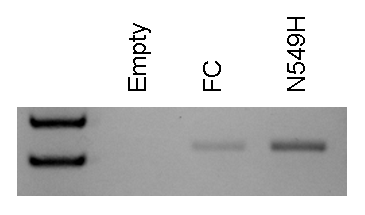
\includegraphics[width=\textwidth,keepaspectratio]{images/240/fusion_rtpcr}
            \caption{}\label{fig:240:fusion_rtpcr}
        \end{subfigure}\par\vspace{0.5cm}
        \begin{subfigure}{\textwidth}
            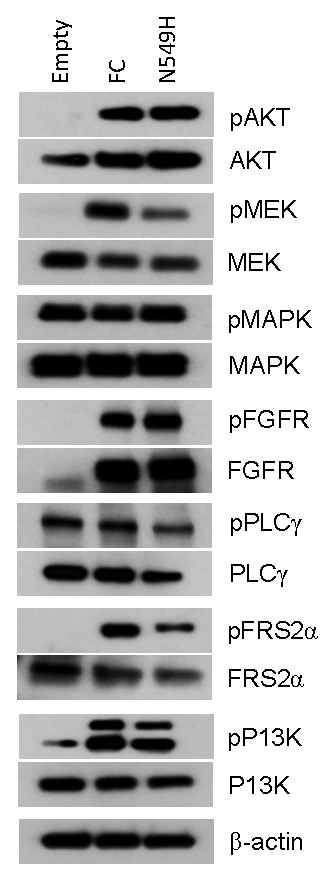
\includegraphics[width=\textwidth,keepaspectratio]{images/240/fusion_downstream_western}
            \caption{}\label{fig:240:fusion_downstream_western}
        \end{subfigure}
    \end{minipage}
    \hfill
    \begin{minipage}[t]{0.73\textwidth}
        \vspace{0pt}
        \begin{subfigure}{\textwidth}
            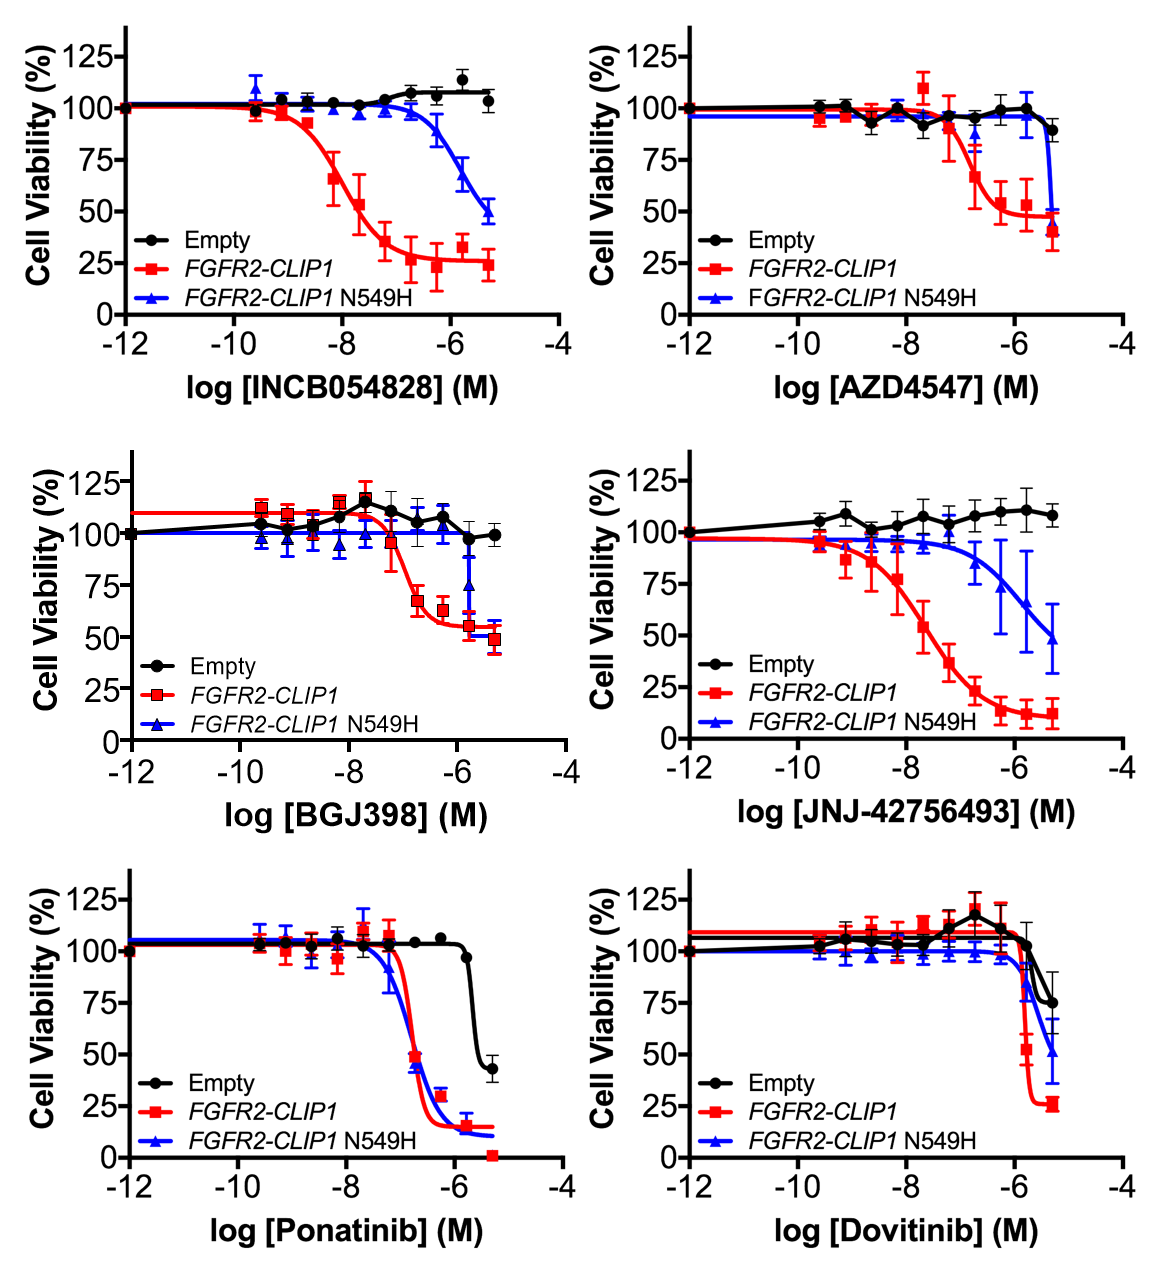
\includegraphics[width=\textwidth,keepaspectratio]{images/240/fusion_ic50_curves}
            \caption{}\label{fig:240:fusion_ic50_curves}
        \end{subfigure}
    \end{minipage}
    \caption[N549H confers FGFR inhibitor resistance to the FGFR2-CLIP1 fusion.]{The FGFR2-CLIP1 fusion is sensitive to FGFR inhibitors whereas the N549H kinase domain mutation confers resistance. (\subref{fig:240:fusion_rtpcr}) RT-PCR confirmed the presence of the FGFR-CLIP1 fusion in the NIH3T3 \textit{FGFR2-CLIP1} (FC) cells and NIH3T3 \textit{FGFR2-CLIP1} N549H (N549H) cells. The fusion was not detected in the control vector (Empty) transduced cells. (\subref{fig:240:fusion_downstream_western}) Total cell lysates from NIH3T3 Empty, FC, and N549H cells were prepared and subjected to Western analysis with antibodies against: pAKT, AKT, pMEK, MEK, pMAPK, MAPK, pFGFR, FGFR, pPLCy, PLC, pFRS2, FRS2, pPI3K, PI3K, and $\beta$-actin. (\subref{fig:240:fusion_ic50_curves}) IC\textsubscript{50} curves of NIH3T3 Empty, FC, and N549H cells treated with FGFR inhibitors. Data from four replicate experiments is shown. Inhibitors include INCB054828, AZD4547, BGJ398 and JNJ42756493, ponatinib and dovitinib. }
    \label{fig:240:fusion_assays}
\end{figure}
To confirm our clinical findings that the FGFR2-CLIP1 fusion is exquisitely sensitive to INCB054828 and explore the hypothesis that the \textit{FGFR2} N549H mutation confers resistance to INCB054828, we generated NIH3T3 cells that express either a control (Empty) vector, \textit{FGFR2-CLIP1} fusion (FC), or \textit{FGFR2-CLIP1} fusion with the N549H secondary mutation (N549H) and confirmed expression by RT-PCR (Figure~\ref{fig:240:fusion_rtpcr}) and Sanger sequencing (data not shown). Western blot analyses of cells expressing the FGFR2-CLIP1 fusion demonstrated increases in PI3K/AKT, MAPK/MEK, and FGFR2 signaling pathways with or without N549H (Figure~\ref{fig:240:fusion_downstream_western}).

\begin{table}[htp]
    \centering
    \begin{tabular}{c:cccccc}
        \multicolumn{1}{c}{~} & \multicolumn{6}{c}{\textbf{IC\textsubscript{50} Values (nM)}} \\
        \hline
        & \rotatebox{270}{\textbf{INCB054828}} & \rotatebox{270}{\textbf{AZD4547}} & \rotatebox{270}{\textbf{BGJ398}} & \rotatebox{270}{\textbf{JNJ-42756493~~}} & \rotatebox{270}{\textbf{Ponatinib}} & \rotatebox{270}{\textbf{Dovitinib}} \\
        \hline
        \textit{FGFR2-CLIP1} & 10.16 & 148.59 & 108.39 & 23.28 & 166.34 & 1548.82 \\
        \textit{FGFR2-CLIP1} N549H & 1527.57 & 4764.31 & 1663.41 & 1355.19 & 162.93 & 2710.19
    \end{tabular}
    \caption[Sensitivity of FGFR2-CLIP1 WT and N549H to FGFR inhibitors.]{Sensitivity of \textit{FGFR2-CLIP1} wild-type and N549H to FGFR inhibitors. IC\textsubscript{50} values are reported for each FGFR inhibitor listed in Figure~\ref{fig:240:fusion_ic50_curves}.}
    \label{table:240:fusion_ic50}
\end{table}
To evaluate the \textit{in vitro} sensitivity of cells with the \textit{FGFR2-CLIP1} fusion and cells with \textit{FGFR2-CLIP1} N549H to the FGFR inhibitor INCB054828, we treated NIH3T3 Empty, \textit{FGFR2-CLIP1}, and \textit{FGFR2-CLIP1} N549H cells with increasing doses of INCB054828 or vehicle control (DMSO) ranging from 1.0 nM~to 5000~nM and assessed cell viability after 72 hours (Figure~\ref{fig:240:fusion_ic50_curves}). Treatment of NIH3T3 \textit{FGFR2-CLIP1} (FC) cells with INCB054828 demonstrated substantial and reproducible inhibition of cell viability with an IC\textsubscript{50} value of 10.16 nM (Table~\ref{table:240:fusion_ic50}). Consistent with our hypothesis, the \textit{FGFR2-CLIP1} N549H (N549H) cells were resistant to INCB054828 with an IC\textsubscript{50} value of 1527.57~nM\@. Empty vector control cells (Empty) were not sensitive to INCB054828, which is expected as these cells do not express endogenous FGF ligands or FGF receptors. Thus, these data help explain this patient's clinical course with his initial \textit{FGFR2-CLIP1} fusion expressing tumor responding to INCB054828 followed by acquisition of resistance via the N549H mutation.

We subsequently extended these \textit{in vitro} studies to include additional FGFR inhibitors that are currently being evaluated clinically in patients with metastatic cancer and have shown early responses in patients with FGFR-mutant cancers (Figure~\ref{fig:240:fusion_ic50_curves}). AZD4547, BGJ398, and JNJ-42756493 are selective FGFR inhibitors, whereas ponatinib and dovitinib are nonspecific tyrosine kinase inhibitors that target BCR-ABL, VEGFR, PDGFR, SRC, RET, KIT, and FLT1 in addition to FGFR\@. Our results demonstrated that FGFR2-CLIP1 cells were sensitive to AZD4547, BGJ398, JNJ-42756493, and ponatinib with IC50 values of 148.59~nM, 108.39~nM, 23.28~nM, and 166.34~nM, respectively (Table~\ref{table:240:fusion_ic50}). The \textit{FGFR2-CLIP1} N549H cells were less sensitive to BGJ398, and AZD4547, JNJ-42756493, as demonstrated by higher IC50 values than the fusion alone. Interestingly, \textit{FGFR2-CLIP1} N549H cells demonstrated similar sensitivity to ponatinib as cells with the fusion alone. Dovitinib was largely ineffective against FGFR2-CLIP1 without or with the secondary mutation. Empty vector control cells (Empty) were not sensitive to AZD-4547, BGJ398, or JNJ-42756493. However, at the highest dose (5~\textmu{}M) of ponatinib and dovitinib, the control cells (Empty) demonstrated decreased cell viability, which was not surprising as ponatinib and dovitinib are non-specific inhibitors of FGFR\@. Taken together, these data demonstrate that the FGFR2-CLIP1 fusion confers sensitivity to some, but not all, FGFR inhibitors. The \textit{FGFR2} N549H secondary mutation confers resistance to most FGFR inhibitors, but ponatinib could be used to overcome this acquired drug resistance.

\section{Discussion}
Tumor heterogeneity has been shown to have a critical role in response to therapy, development of resistance, and clinical outcome in patients with cancer \cite{choi2017,joung2017,rottenberg2012}. Rapid research autopsy has emerged as a powerful strategy to study tumor heterogeneity, as it enables essentially unlimited sampling of all sites of metastatic disease throughout the body which would otherwise not be feasible through surgical resections or tumor biopsies \cite{krook2019_review}. A number of recent studies have utilized rapid research autopsy to characterize tumor heterogeneity, clonal evolution, and mechanisms of acquired therapeutic resistance in breast, urothelial, pancreatic, and colorectal cancer. For instance, Saito \textit{et al} utilized research autopsy in breast cancer to assess trastuzumab resistance in primary versus metastatic sites \cite{saito2015}. Faltas \textit{et al} performed rapid autopsy of two patients to construct phylogenetic trees of urothelial carcinoma \cite{faltas2016}. Here, we present our findings from rapid research autopsy of a patient with metastatic cholangiocarcinoma. This is the first study to evaluate clonal heterogeneity based on exome sequencing in cholangiocarcinoma, as well as the first description of acquired resistance to INCB54828, an oral FGFR inhibitor.

Most previous and current autopsy studies utilize methods such as clonal ordering \cite{merlo2006} and neighbor joining (NJ) \cite{saitou1987} to identify and quantify relationships between different tumor regions and/or sites of metastatic cancer. In this study, we utilized the NJ method to generate a tumor-centric tree to assess similarities and differences among the pre-treatment biopsy, post-progression biopsy and nine unique tumors collected at the time of autopsy. The NJ analysis showed that the liver \#1 sample with its unique \textit{FGFR2} N549H point mutation is an outlier versus the other liver samples from autopsy. NJ and related phylogenetic methods are powerful tools to assess high-level relatedness among tumors and identify exceptional tumors, however they cannot capture the clonal heterogeneity present within discrete tumor masses or cross-seeding between sites.

Analysis of clonal evolution continues to develop as technical and computational challenges and the limited availability of large-scale autopsy data are overcome. In addition to neighbor joining, we performed subclonal inference using Canopy \cite{canopy}, which revealed 4 genetically distinct tumor subclones. Of these subclones, three were dominant across all 11 samples, with each subclone characterized by a specific set of mutations (Figure~\ref{fig:240:canopy_results}). The \textit{FGFR2} N549H mutation in clone 1 was unique to a single liver sample despite our in vitro data confirming its role as a resistance mutation. This pattern of site-unique \textit{FGFR2} resistance mutations was previously observed by Goyal \textit{et al} \cite{goyal2017} in which only 4 of 12 distinct metastatic autopsy samples were found to have acquired secondary mutations in \textit{FGFR2} serving to bypass the FGFR inhibitor effect. Each of these samples harbored unique \textit{FGFR2} mutations (K641R and N549H) with only one sample having two \textit{FGFR2} mutations (E565A and K641R)\@.  Meanwhile, the remaining 8 sites were wild-type for \textit{FGFR2}. The observations seen by Goyal \textit{et al} along with our work presented here, suggest that multiple independent drug resistance mechanisms, including FGFR-independent mechanisms, are likely contributing to tumor progression. Interestingly, in our model, clone 4 was specific to tumor samples collected at the time of autopsy, suggesting that either the biopsies missed a population of cells or that this subclone developed after the post-treatment biopsy. FOLFOX was administered after the collection of the post-treatment biopsy, but as this patient only received one dose of FOLFOX before passing away soon afterwards, we do not believe that this single dose substantially affected the heterogeneity present at time of autopsy. These findings provide evidence for the presumed notion that tumor biopsies do not accurately reflect the full complexity and heterogeneous nature of the disease. Clones 2 through 4 were seen in all autopsy samples at similar proportions. As the liver tumors were largely confluent at time of autopsy (Figure~\ref{fig:240:autopsy_gross}), multiple samples may have come from the same tumor. Another possibility is metastatic cross-seeding, as was observed by Savas \textit{et al} \cite{savas2016} using their tool superFREQ \cite{flensburg2020} for subclonal analysis of four metastatic breast cancer cases, and by Brady \textit{et al} \cite{brady2019} in pediatric osteosarcoma. Co-metastasis of multiple subclonal populations can also explain this distribution, as has been demonstrated to occur in breast ductal carcinoma \cite{casasent2018}. Clone 2 was substantially reduced in the post-treatment and autopsy samples vs.\ the pre-treatment biopsy. One potential explanation is that clone 2 was more sensitive to INCB054828 than clones 1, 3 and 4. In clone 1, the decreased sensitivity is likely due to the \textit{FGFR2} N549H point mutation, evolving from a common lineage as clone 2. Although resistance mechanisms for clones 3 and 4 could not be determined through whole exome sequencing, and driver prediction did not indicate any other likely driver mutations, we hypothesize that there can be multiple independent drug resistance adaptations within a single patient. Previous studies have demonstrated that in addition to secondary kinase domain mutations, activation in the Akt, MAPK, and PTEN pathways can mediate resistance to FGFR inhibition \cite{datta2017,goyal2017,malchers2017}. While there was no evidence for \textit{PTEN} mutations in this patient, transcriptome sequencing would be needed to assess activation of other pathways. Studies are ongoing in our laboratory to identify FGFR-independent mechanisms of resistance and to define their contributions clinically, including by RNA sequencing.

Whole exome sequencing of this patient and derivation of a phylogenetic tree suggests that ancestral genotypes can persist throughout the disease course, despite the evolution of highly derived subclones. We note that only four SNVs, three indels, and one copy number gain were detected in the trunk of this patient's phylogenetic tree (branch \textbf{\textit{a}}), indicating that development of \textit{FGFR2} fusion-positive cholangiocarcinoma may only require a small number of other initiating events (Figure~\ref{fig:240:canopy_tree}). For instance, clone 4 was only detected in autopsy samples, yet evolved from a distant ancestor to clones 1, 2 and 3. Clone 1 did not directly evolve from clone 2, but rather it shares a common ancestor with clone 2 which must have been extant before treatment (for clone 2 to be found in the pre-treatment sample). Such persistent ancestral cells may serve as an ``uncommitted'' tumor reserve capable of developing new adaptations throughout the disease course. Subclonal analysis, such as in this study, permits characterization of cancer as a dynamic process of multiple evolving and diverging cellular populations rather than a singular entity in a patient. This view of cancer permits somatic variants, a staple of cancer genomics, to be viewed in a new context. However, phylogeny inference from short-read bulk sequencing has several inherent limitations, most notably that phylogenetic solutions consistent with variant fractions and CNVs are frequently non-unique \cite{pradhan2018}. Emerging long-read and single-cell sequencing technologies will permit more certain and accurate modeling of phylogeny by directly assessing the phasing of subclonal mutations.

Lessons learned from studying molecular mechanisms of resistance to ABL, EGFR, ALK, KIT, and RAF inhibitors in human cancers have highlighted the need for next generation kinase inhibitors that are effective against acquired secondary resistance mutations \cite{demetri2011,gainor2013,hrustanovic2015,lito2013,roychowdhury2011_cml,vanallen2014}. For example, Friboulet \textit{et al} demonstrated that crizotinib induced resistance mutations in ALK-fusion positive non-small cell lung cancer (NSCLC) can be overcome by treatment with ceritinib \cite{friboulet2014}. Furthermore, mutant-selective allosteric inhibitors have shown promise in overcoming the secondary \textit{EGFR} resistance mutation T790M in NSCLC following EGFR-directed therapy \cite{jia2016}. Thus, these studies may inform strategies to overcome secondary resistance mutations to FGFR targeted therapies as several preclinical studies have demonstrated the emergence of a mutation at the gatekeeper residue or other residues within the ATP-binding pocket as well as other mutations in \textit{FGFR1--3} \cite{chell2013}. Unfortunately, several potent and selective ATP-competitive small molecule FGFR inhibitors currently in clinical trials, including INCB054828, BGJ398, AZD4547, and LY2874455, share structural similarities and are ineffective in overcoming the gatekeeper mutations \cite{chae2017}. While not considered a gatekeeper mutation, the \textit{FGFR2} N549H mutation is in the vicinity of the ATP binding pocket. Notably, our in vitro findings provide further support for the cross-resistance of multiple FGFR inhibitors, as cells harboring the secondary \textit{FGFR2} mutation N549H were resistant to INCB054828, AZD4547, BGJ398, JNJ-42756493, and dovitinib. Because of this, there has been interest in the use of structure-based drug design to develop a class of next-generation inhibitors that would overcome resistance mutations located in the FGFR2 ATP-binding pocket \cite{tan2014}. Interestingly, we demonstrated that \textit{FGFR2} N549H retained sensitivity to ponatinib. The clinical use of ponatinib in this context is supported by pharmacokinetic data in patients demonstrating a steady state ponatinib plasma concentration of 145 nM attained 4--8 hr after receiving the maximum approved dose of 45 mg \cite{cortes2012}. Unfortunately, there are serious adverse cardiovascular events associated with ponatinib, which are often dose-limiting \cite{nicolini2013}. Thus, the development of next-generation FGFR inhibitors has the potential to dramatically impact the clinical care of patients receiving FGFR targeted therapies.

In summary, this work suggests that clonal heterogeneity contributes to acquired clinical resistance to the novel FGFR inhibitor, INCB054828, in cholangiocarcinoma. Though limited to a single patient, this is the first study, to our knowledge, to define a mechanism of acquired resistance to INCB054282 through a secondary mutation to the FGFR inhibitor, INCB054828. Through rapid research autopsy and whole exome sequencing, we determine the presence of four tumor subclones and elucidate their evolution in metastatic tissues over time in a patient with FGFR2-fusion positive cholangiocarcinoma. Furthermore, we identified a post-treatment secondary kinase mutation in \textit{FGFR2}, present in a single metastatic tumor sample demonstrating the significance of intertumor heterogeneity within the same patient. We characterized the impact of the N549H mutation on sensitivity to different FGFR inhibitors \textit{in vitro}. The results of our \textit{in vitro} drug sensitivity studies suggest that this mutation conferred resistance to INCB054828 in this patient and thus may have potential as a clinically useful biomarker of resistance. Overall, our findings suggest that secondary FGFR mutations are drivers of acquired clinical resistance. Understanding these mechanisms of resistance along with FGFR kinase domain-independent mechanisms of resistance will facilitate approaches to prevent or overcome treatment resistance and disease recurrence and guide clinical strategies for these patients.

\section{List of Supplemental Files}
All supplemental files are available at \url{https://github.com/rbonneville/PhD-Dissertation/}.
\begin{enumerate}
    \renewcommand*{\labelenumi}{S\thechapter{}.\arabic{enumi}. }
    \item Annotated somatic mutations identified in each tumor sample. SNVs and indels were called with VarScan2 (Section~\ref{ssec:240:alignment_variant_calling}). Annotation was performed using ANNOVAR.
    \item Mutational signatures per tumor sample. Mutational signatures within the COSMIC Mutational Signatures set were called using deconstructSigs.
    \item Raw allele-specific CNA calls in each tumor sample. Copy number variations were called using FALCON.
    \item Manually curated CNA calls per tumor sample. Major CN corresponds to $\mathbf{W}_M$ in Canopy, minor CN to $\mathbf{W}_m$, major SD to $\mathbf{\varepsilon}_M$, and minor SD to $\mathbf{\varepsilon}_m$.
    \item Estimated subclonal composition of each tumor sample. Normal represents the estimated proportion of non-tumor cells in each sample.
    \item SNVs and indels were called with VarScan2 (Section~\ref{ssec:240:alignment_variant_calling}). Annotation was performed using ANNOVAR. ``post-progression + autopsy uniq'' contains mutations unique to the post-progression and autopsy samples (\textit{i.e.}\ absent in the pre-treatment sample), and ``autopsy unique'' contains mutations found in at least one autopsy sample but not the pre-treatment or post-progression biopsies.
    \item Each branch (\textbf{\textit{a--f}}) corresponds to a branch in Figure~\ref{fig:240:canopy_tree}. Columns C--M contain the variant fraction of each mutation in each sample, and column N contains the estimated ability score of each mutation. Higher ability scores correspond to predicted earlier development of the mutation (Section~\ref{ssec:240:subclonal_inference}).
    \item Each branch (\textbf{\textit{a--f}}) corresponds to a branch in Figure~\ref{fig:240:canopy_tree}. Note that region \texttt{chr8\_c} (chr8:124448804--146364022) had two separate copy number variations, one in branch \textbf{\textit{a}} and the other in branch \textbf{\textit{c}}.
    \item Driver mutation prediction with CHASM\@. Predicted driver mutations are indicated with CHASM FDR $\le 0.05$.
\end{enumerate}

\section*{Acknowledgements}
We would like to thank Jenny Badillo for her administrative support. We would also like to thank current and past members of the Roychowdhury Precision Cancer Medicine Team, The Ohio State Comprehensive Cancer Center, James Cancer Hospital, and community support from Pelotonia. We would most importantly like to thank this patient and his family. We would also like to thank the Ohio Supercomputer Center for computing resources.

Data used for the analyses presented in this study have been submitted to dbGaP (\url{https://ncbi.nlm.nih.gov/gap}) under the project accession number phs001830.v1.p1. The \textit{FGFR2-CLIP1} fusion gene variant and the secondary \textit{FGFR2} mutation identified in the patient have been deposited to ClinVar (\url{https://ncbi.nlm.nih.gov/clinvar/}) under the accession numbers SCV000927106 and SCV000914229.1, respectively.
